% Select one class
%\documentclass{pucthesis}		% For DVI
\documentclass[pdftex,spanish]{pucthesis}	% For pdfLaTeX, en espa\~nol

%%%%%%%%%
%   Packages	 %
%%%%%%%%%

% Floats
\usepackage{graphicx}
\usepackage{float}
\usepackage{subfigure}
\usepackage[table]{xcolor}

% Math packages
\usepackage{amsmath}
\usepackage{amsfonts}
\usepackage{amssymb}

% To make pretty tables
\usepackage{booktabs}
\usepackage{multirow}

% To avoid underfull errors in the bibliography
\usepackage{etoolbox}
\apptocmd{\sloppy}{\hbadness 10000\relax}{}{}

% To make cites and references
\usepackage[hidelinks,pdfusetitle,pdfdisplaydoctitle]{hyperref}
\usepackage[notocbib]{apacite}
\usepackage{doi}
\renewcommand{\doitext}{}

%--------- Cuerpo del texto en Times 11pt (la clase carga amsbook en 12pt) ---------
% Los Lineamientos de la Entrega exigen Times New Roman 11pt. La clase pucthesis
% ya usa mathptmx (Times) mediante \LoadClass[...,12pt]{amsbook}; aqu\'i solo se
% redefine \normalsize a 11pt sin tocar pucthesis.cls, como recomienda su README.
\makeatletter
\renewcommand{\normalsize}{%
  \@setfontsize\normalsize\@xipt{13.6}%
  \abovedisplayskip 11\p@ \@plus3\p@ \@minus6\p@
  \abovedisplayshortskip \z@ \@plus3\p@
  \belowdisplayshortskip 6.5\p@ \@plus3.5\p@ \@minus3\p@
  \belowdisplayskip \abovedisplayskip
  \let\@listi\@listI}
\normalsize
\makeatother

% Colores usados en la Carta Gantt (Cap\'itulo de Conclusiones)
\definecolor{ganttgreen}{HTML}{4EA72E}

% Filas de tablas levemente m\'as compactas (sin quitar columnas ni datos)
\renewcommand{\arraystretch}{0.9}

\begin{document}

% Interlineado levemente m\'as compacto que el 1.5 por defecto de la clase
% (pucthesis.cls ya carga el paquete setspace, se usa \setstretch en vez de
% tocar el .cls directamente).
\setstretch{1.4}

\mdate{Septiembre 2026}         % date manuscript changed
\version{1}                                     % manuscript version #

\title[PLANIFICACI\'ON DE LA OPERACI\'ON DE LOS BUSES EL\'ECTRICOS\\ EN LA RED METROPOLITANA DE MOVILIDAD DE SANTIAGO\\ GRUPO 24]
   {\bf PLANIFICACI\'ON DE LA OPERACI\'ON DE LOS BUSES EL\'ECTRICOS\\ EN LA RED METROPOLITANA DE MOVILIDAD DE SANTIAGO\\ GRUPO 24}
\author[Integrantes:]{Integrantes:\\
\textnormal{\small{
Nicol\'as Bennett\\
Antonio De Frutos\\
Claudio Hasb\'un\\
Agust\'in Irarr\'azaval\\
Joaqu\'in Jim\'enez\\
Alonso Muelas}
}
}

\address{Escuela de Ingenier\'ia\\
                   Pontificia Universidad Cat\'olica de Chile\\
                   Vicu\~na Mackenna 4860\\
                  Santiago, Chile\\
                  {\it Tel.\/} : 56 (2) 354-2000}


\advisor                    {\textbf{Profesor Gu\'ia:} Agust\'in Chiu}
\ogrsmember                 {\textbf{Ayudante Tutor:} Max Burr}
\date                                 {Septiembre 2026}
\copyrightname             {Grupo 24}
\copyrightyear               {2026}

%%%%%%%%%%%%%%%%%%%%
%       PRELIMINARIES                              %
%----------------------------------------------------%
%      page i & ii: cover page                   %
%%%%%%%%%%%%%%%%%%%%

\NoChapterPageNumber
\pagenumbering{roman}
\maketitle

%----------------------------------------------------------------------%

%%%%%%%%%%%%%%%%%%
%          page v & up ---                      %
%            Table of contents              %
%            List of figures                     %
%            List of tables                      %
%%%%%%%%%%%%%%%%%%

\pdfbookmark{\contentsname}{toc}
\tableofcontents
\phantomsection \label{listoffigures}
\listoffigures
\phantomsection \label{listoftables}
\listoftables
\cleardoublepage

%----------------------------------------------------------------------%

%%%%%%%%%%%%%%%%%%%%%%%%
%      RESUMEN        %
%%%%%%%%%%%%%%%%%%%%%%%%

\phantomsection \label{resumen}
\chapter*{RESUMEN}
En este proyecto se estudia el problema de asignar los viajes de RED a una flota de buses el\'ectricos, determinando simult\'aneamente sus secuencias de operaci\'on y necesidades de recarga, con el objetivo de minimizar los costos operacionales y asegurar que todos los viajes sean cubiertos de manera factible.

Como primera aproximaci\'on, se analizan los datos disponibles de rutas, expediciones, horarios, paraderos, caracter\'isticas de los buses, electroterminales y tarifas el\'ectricas, considerando inicialmente un d\'ia laboral, que concentra 417 rutas y 64.502 expediciones. A partir de la revisi\'on bibliogr\'afica se estudian distintas metodolog\'ias de resoluci\'on, entre ellas Adaptive Large Neighborhood Search, Set Partitioning con Generaci\'on de Columnas y cortes de Benders, y una estrategia de descomposici\'on espaciotemporal. Esta \'ultima se propone como enfoque principal, al dividir el problema primero por electroterminal y posteriormente mediante ventanas horarias superpuestas, reduciendo la escala de los subproblemas a resolver. El presente informe corresponde a una etapa preliminar del proyecto, por lo que se establecen las bases del modelo, los indicadores de desempe\~no y las metodolog\'ias que ser\'an implementadas y evaluadas en las siguientes etapas.

\vfill
\noindent {\bf Palabras Clave}: Electric Vehicle Scheduling Problem, buses el\'ectricos, RED Metropolitana de Movilidad, programaci\'on de recargas, descomposici\'on espaciotemporal, optimizaci\'on de flotas.

\cleardoublepage

%%%%%%%%%%%%%
%   TEXT  OF THESIS     %
%%%%%%%%%%%%%

\pagenumbering{arabic}

\chapter[INTRODUCCI\'ON]{Introducci\'on}
En los \'ultimos a\~nos, la electromovilidad se ha consolidado como uno de los pilares de la transformaci\'on hacia sistemas de transporte p\'ublico m\'as limpios y sostenibles, en un contexto de creciente preocupaci\'on por el cambio clim\'atico y la calidad del aire en las ciudades. Chile no ha sido ajeno a este proceso. Desde la llegada de los primeros buses el\'ectricos a Santiago a fines de 2018 \cite{worldbank2020}, el pa\'is ha avanzado hacia la electrificaci\'on de su transporte p\'ublico para enfrentar el hist\'orico problema de contaminaci\'on atmosf\'erica de la capital, reduciendo emisiones y ruido. Sin embargo, la incorporaci\'on de flotas el\'ectricas no es un reemplazo directo de la tecnolog\'ia convencional, ya que introduce restricciones operacionales nuevas que exigen repensar c\'omo se planifica la operaci\'on diaria. La Red Metropolitana de Movilidad (RED) de Santiago es uno de los sistemas de transporte p\'ublico m\'as grandes de Am\'erica Latina y cuenta con la flota de buses el\'ectricos m\'as grande fuera de China, lo que convierte a Santiago en un caso de estudio a escala real, con la complejidad operacional propia de una red metropolitana masiva.

La complejidad de incorporar buses el\'ectricos a un sistema planificado para buses di\'esel radica en que estos veh\'iculos no operan bajo la misma l\'ogica que sus predecesores. Un bus el\'ectrico tiene una autonom\'ia considerablemente menor por la limitaci\'on de su bater\'ia, que necesita tiempos de recarga considerables (de noche en los dep\'ositos o en pausas operacionales durante el d\'ia) y solo puede recargarse en electroterminales, instalaciones a\'un escasas y con pocos cargadores. Esto convierte la planificaci\'on en un problema conjunto de transporte y energ\'ia, donde adem\'as de asignar buses a los viajes debe decidirse cu\'ando y d\'onde recargar cada veh\'iculo sin saturar una infraestructura compartida y limitada. Frente a esta complejidad, la Investigaci\'on Operativa ofrece las herramientas adecuadas para abordar el problema mediante la optimizaci\'on matem\'atica, las heur\'isticas, la simulaci\'on y el an\'alisis de datos que permiten explorar sistem\'aticamente distintas estrategias de operaci\'on y evaluar su costo y desempe\~no.

En el resto de este informe se presenta una primera aproximaci\'on al problema de planificaci\'on operacional de la flota el\'ectrica de RED, donde se describe en detalle el problema abordado, se analizan los datos disponibles junto con los indicadores de desempe\~no considerados y se discuten las metodolog\'ias de resoluci\'on candidatas.


\chapter[DESCRIPCI\'ON DEL PROBLEMA]{Descripci\'on del Problema} \label{ch:problema}
\section{Problema \label{sec:problema}}

El problema que presenta la red de transporte el\'ectrica de buses RED es uno del tipo ``Electric Vehicle Scheduling Problem'', es decir un problema de asignaci\'on de veh\'iculos con estaciones de carga el\'ectricas. Se dispone de un conjunto de viajes programados que deben ser cubiertos durante un d\'ia de operaci\'on, cada uno definido por un paradero y hora de inicio, un paradero y hora de t\'ermino, paraderos intermedios, distancia recorrida y consumo energ\'etico asociado. Estos viajes deben asignarse a una flota de buses homog\'enea irrestricta, con un costo fijo diario por activaci\'on operacional de cada bus, de manera que cada viaje sea atendido una vez y que la secuencia asignada a cada bus constituya una cadena operacional f\'isicamente factible, es decir, un bus solo puede iniciar un viaje si tiene el tiempo suficiente para trasladarse, sin pasajeros, desde el punto donde finaliz\'o su ruta anterior hasta el inicio de la nueva. A esto se suma la autonom\'ia limitada de la bater\'ia, que debe mantenerse entre un nivel de carga m\'inimo y m\'aximo, obligando al bus a recargarse en electroterminales antes de que su carga sea cr\'itica. Estos electroterminales presentan, adem\'as, una infraestructura limitada para un n\'umero m\'aximo de buses recarg\'andose simult\'aneamente.

Dado lo anterior, se tienen tres decisiones que se deben tomar en el problema. Primero, la asignaci\'on de viajes a buses, que determina qu\'e bus ejecuta cada viaje y en qu\'e orden. Segundo, los desplazamientos sin pasajeros asociados a dicha asignaci\'on, que incluyen el trayecto de salida desde un electroterminal hacia el primer viaje del turno (\emph{pullout}), el trayecto de regreso desde el \'ultimo viaje hacia un electroterminal (\emph{pullin}), y los desplazamientos entre el t\'ermino de un viaje y el inicio del siguiente cuando ambos no son geogr\'aficamente contiguos. A estos eventos se les denomina \emph{deadheading} (o \emph{deadheads}) y tienen un costo asociado por km recorrido. Por \'ultimo, las decisiones de recarga, que implican el cu\'ando, en qu\'e electroterminal y por cu\'anto tiempo debe recargarse cada bus, sujeto a la capacidad simult\'anea de cada instalaci\'on y a que el costo de la energ\'ia var\'ia seg\'un el bloque horario en que se realice la carga.

\section{Objetivos \label{sec:objetivos}}

Con el contexto del problema ya visto, el objetivo del problema es minimizar el costo total de operaci\'on, compuesto por el costo fijo asociado al n\'umero de buses utilizados diariamente, el costo variable de los desplazamientos sin pasajeros, el costo asociado a los tiempos de espera de los buses, el costo energ\'etico de las recargas y el costo fijo asociado a cada evento de carga, sujeto a que todos los viajes programados sean cubiertos, a la factibilidad temporal y energ\'etica de la secuencia de actividades de cada bus, y a la capacidad de carga simult\'anea de los electroterminales.

\section{Entregable \label{sec:entregable}}

El entregable del proyecto es un plan operacional diario para un d\'ia laboral representativo de la red, compuesto por los siguientes elementos concretos:

\begin{itemize}
\item N\'umero m\'inimo de buses necesarios para cubrir la totalidad de las expediciones programadas.
\item Jornada operacional completa de cada bus en un archivo CSV, es decir, la secuencia ordenada de viajes que le son asignados junto con sus horarios de inicio y t\'ermino, el trayecto de \emph{pullout} desde el electroterminal de salida, los eventuales desplazamientos de \emph{deadheading} entre viajes no contiguos, y el trayecto de \emph{pullin} de regreso a un electroterminal.
\item Itinerario de recarga para cada bus en un archivo CSV, especificando en qu\'e electroterminal, en qu\'e bloque horario y por cu\'anta energ\'ia se recarga, de manera que se respeten el nivel m\'inimo de bater\'ia, la capacidad de los electroterminales y el resto de las restricciones de recarga.
\item Desglose del costo total de la soluci\'on en sus componentes (costo fijo de flota, costo de desplazamientos vac\'ios, costo de tiempos de espera, costo energ\'etico y costo fijo por evento de carga).
\end{itemize}

\section{An\'alisis de Datos \label{sec:analisisdatos}}

\subsection{Datos Disponibles \label{sec:datosdisponibles}}

Los datos utilizados provienen de tres fuentes: un archivo GTFS de RED (vigente julio-diciembre 2026) con las rutas, viajes programados, horarios, paraderos y trazados geom\'etricos de la red; un GeoPackage de OpenStreetMap con la geometr\'ia y atributos de todas las calles de Chile (nombre, tipo de v\'ia, sentido, etc.), usado para calcular distancias sin pasajeros; y un conjunto de archivos CSV con par\'ametros espec\'ificos del proyecto (ubicaci\'on y capacidad de los cinco electroterminales, potencia de los cargadores, precios de electricidad por bloque horario, caracter\'isticas t\'ecnicas del bus el\'ectrico y costos de operaci\'on). El Anexo 2 detalla cada archivo, su contenido y el uso que se le dar\'a en el proyecto.

\subsection{Filtros y Limpieza \label{sec:filtroslimpieza}}

Del archivo GTFS se conservaron \'unicamente las rutas operadas por RED, excluyendo Metro (L1 a L6), Metrotren (MTN y MTR) y una ruta de un operador externo al aeropuerto (BA), junto con sus columnas exclusivas. El feed distingue tres tipos de d\'ia (laboral, s\'abado y domingo); se filtr\'o el laboral como caso base por ser el de mayor exigencia operacional, con la mayor cantidad de rutas activas (417) y de expediciones (64.502), como muestra la Figura \ref{fig:tipodia}.

\begin{figure}[htb]
	\begin{center}
	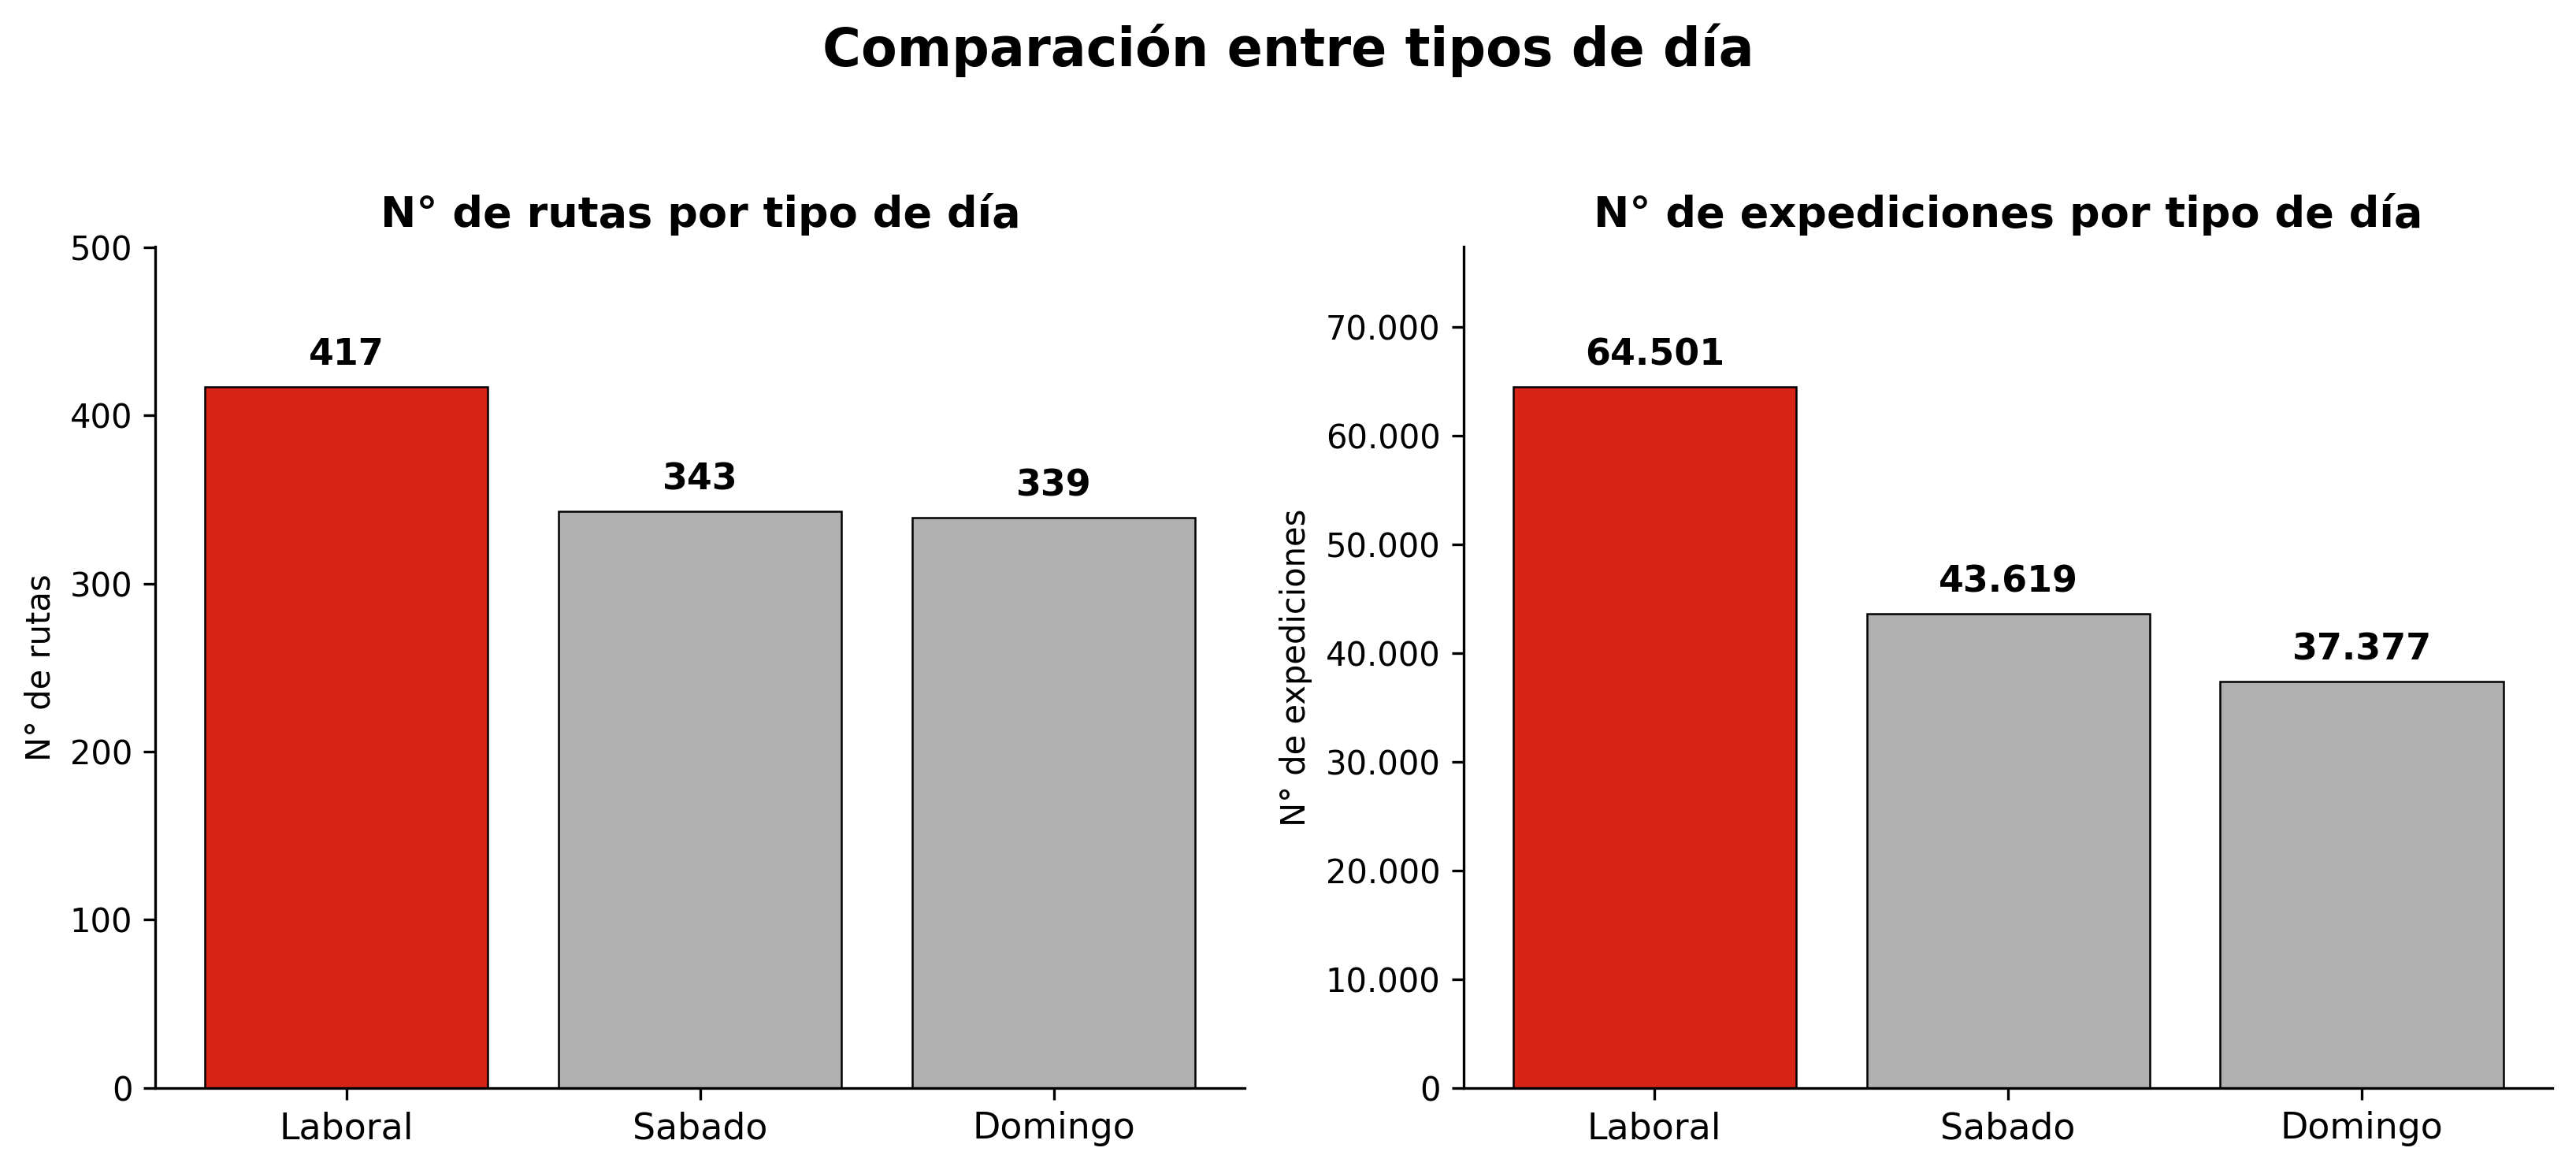
\includegraphics[width=0.65\textwidth]{./figures/grafico_tipo_dia.png}
	\caption[Comparaci\'on entre tipos de d\'ia]{Comparaci\'on entre tipos de d\'ia (n\'umero de rutas y expediciones)}
	\label{fig:tipodia}
	\end{center}
\end{figure}

Una vez filtradas las rutas de RED en d\'ias laborales, la Figura \ref{fig:mapared} muestra el mapa de las rutas que recorrer\'an los buses y la ubicaci\'on de los electroterminales donde deber\'an recargar sus bater\'ias.

\begin{figure}[htb]
	\begin{center}
	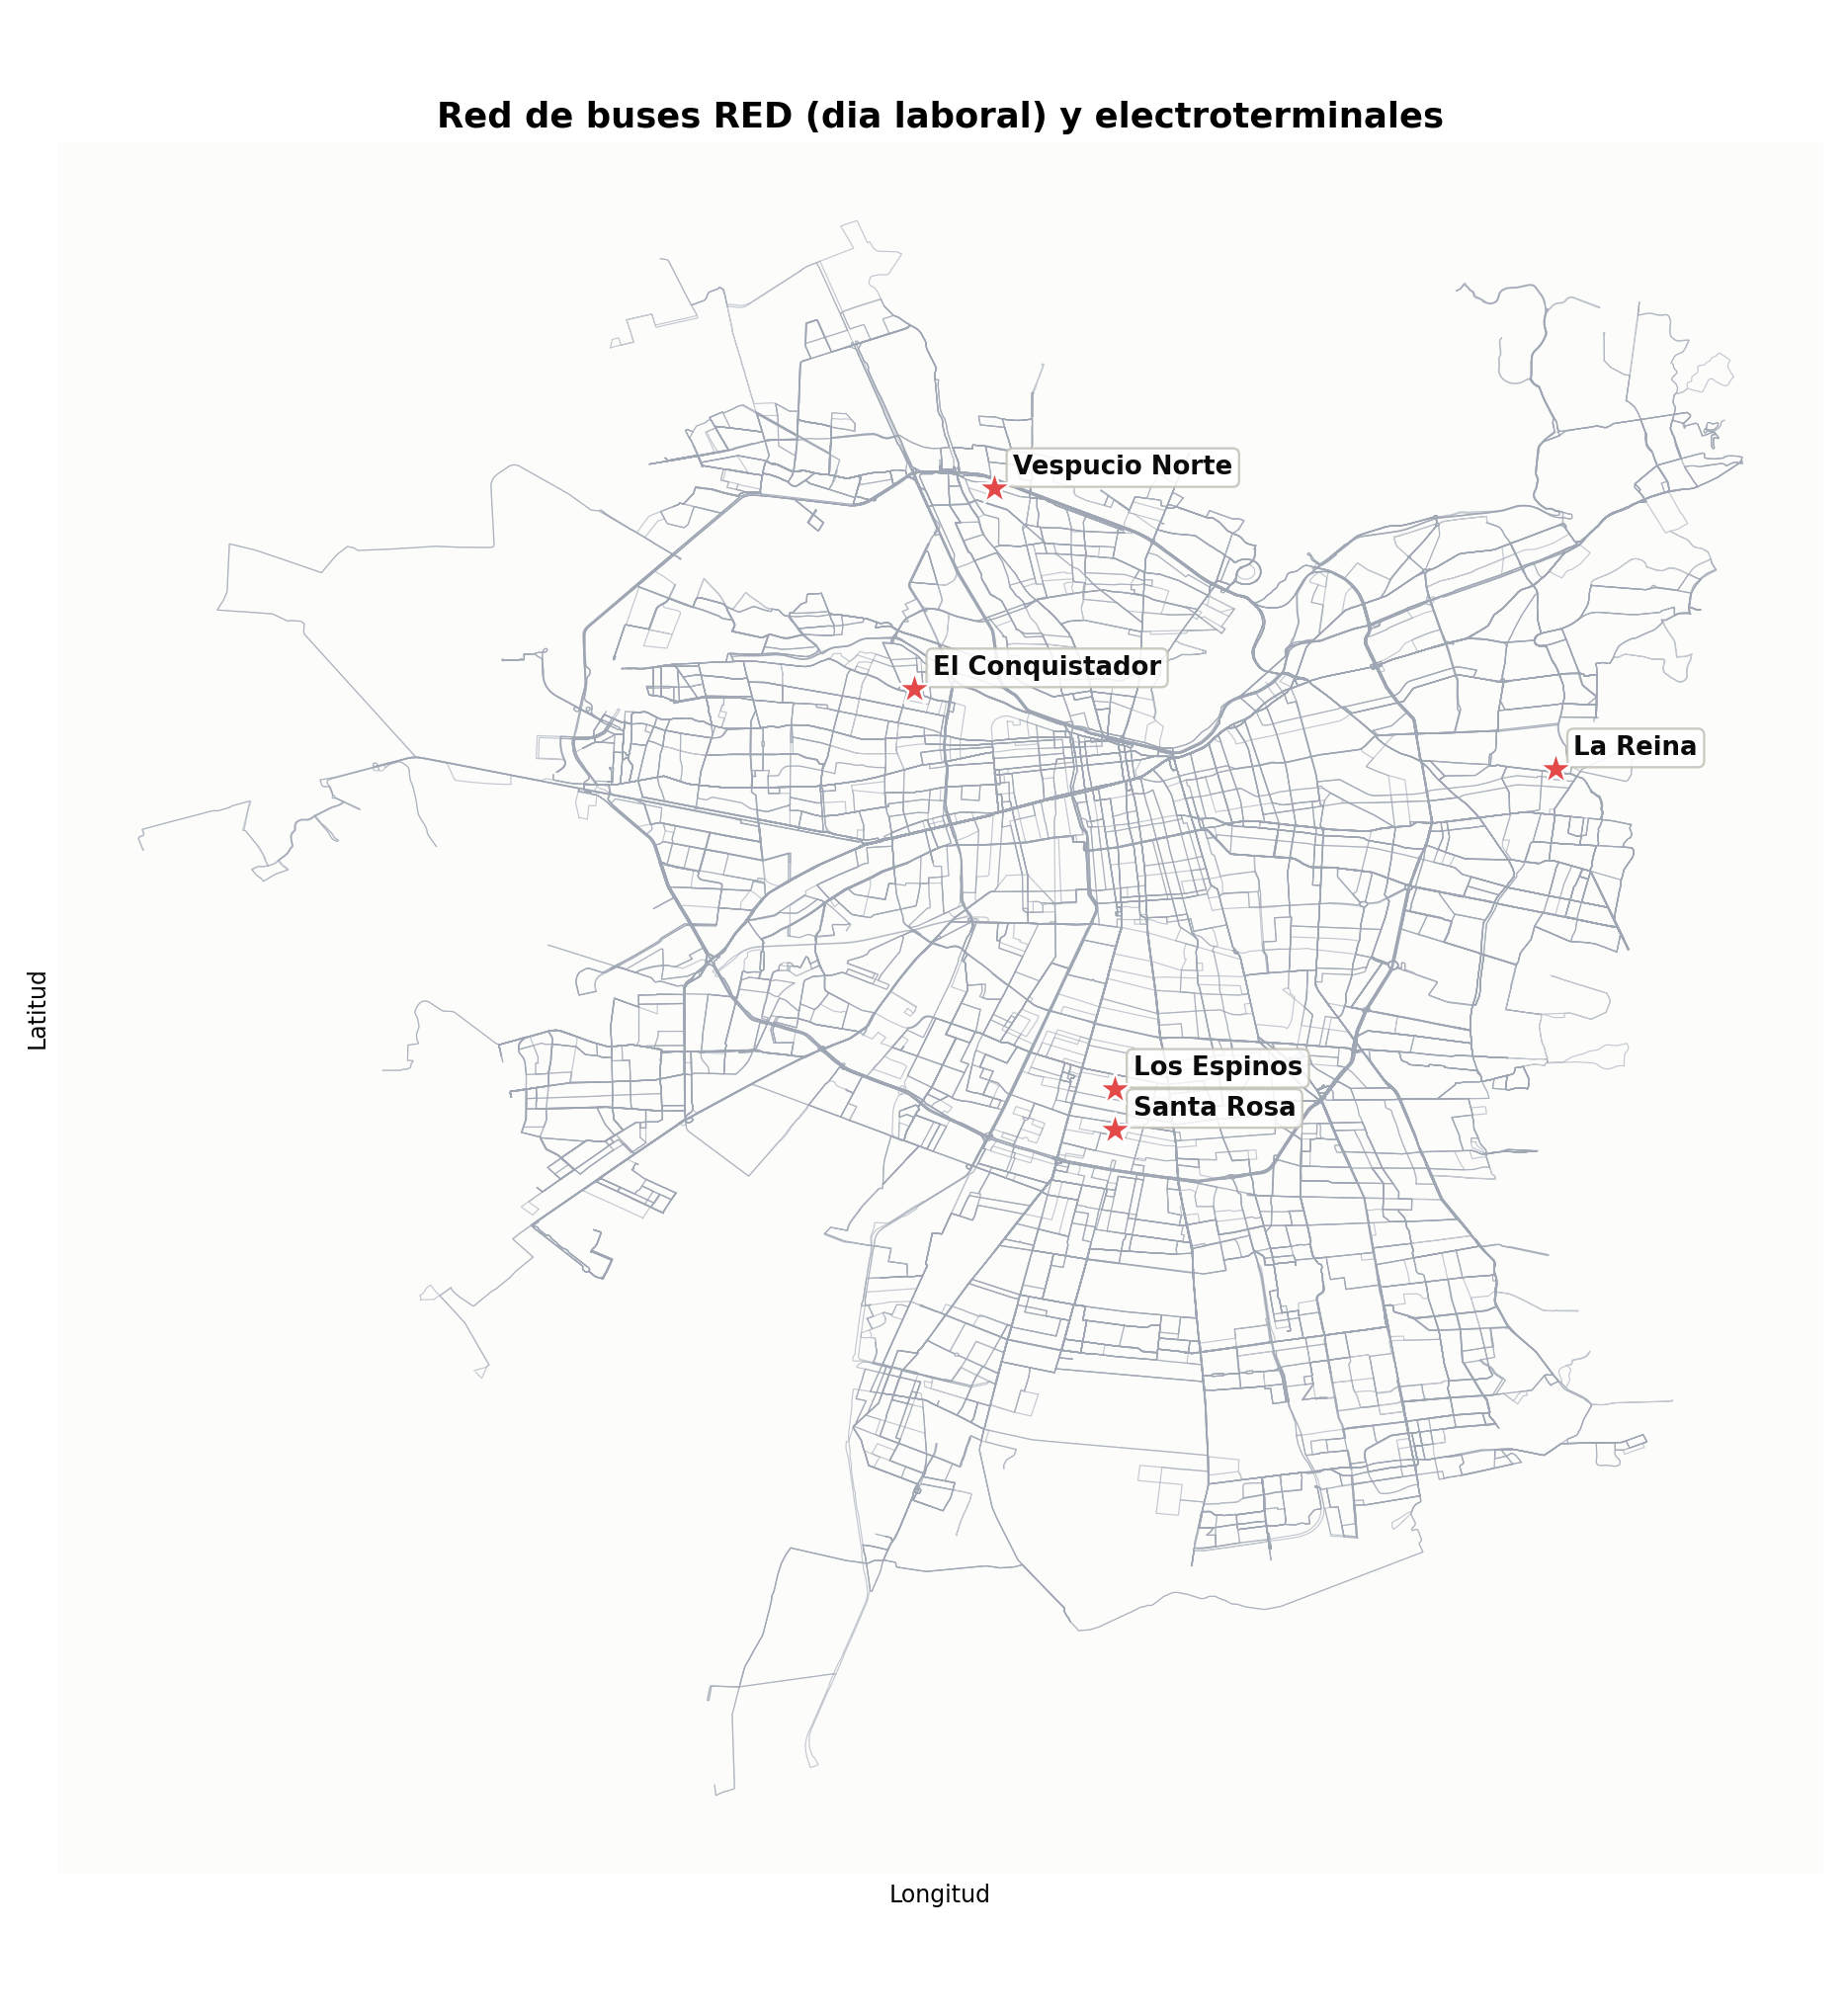
\includegraphics[width=0.5\textwidth]{./figures/mapa_rutas_electroterminales.png}
	\caption[Red de buses RED y electroterminales]{Red de buses RED (d\'ia laboral) y electroterminales}
	\label{fig:mapared}
	\end{center}
\end{figure}

El feed GTFS filtrado a RED y al d\'ia laboral contiene 417 rutas, 839 trazados geom\'etricos, 12.132 paraderos y 6.620 viajes. Al expandir estos viajes por las frecuencias definidas en el archivo \texttt{frequencies}, se obtienen 64.502 expediciones reales que deben ser cubiertas durante el d\'ia. La Tabla \ref{tab:cifrasclave} resume estas cifras.

\begin{table}[htb]
\begin{center}
\small
\caption[Cifras clave de la operaci\'on programada]{Cifras clave de la operaci\'on programada (d\'ia laboral)}
\label{tab:cifrasclave}
\begin{tabular}{@{}l r@{}}\toprule
\textbf{Indicador} & \textbf{Cantidad} \\ \midrule
Rutas & 417 \\
Trazados geom\'etricos & 839 \\
Paraderos & 12.132 \\
Viajes & 6.620 \\
Expediciones & 64.502 \\
\bottomrule
\end{tabular}
\end{center}
\end{table}

La distribuci\'on horaria de estas expediciones no es constante a lo largo del d\'ia. La Figura \ref{fig:busesporhora} muestra la cantidad de buses circulando al mismo tiempo hora a hora, donde se observan dos claros picos de demanda. El primero a las 8:00 con 6.601 buses circulando, correspondiente a entradas a oficinas y establecimientos educacionales. El segundo ocurre a las 18:00 con 6.523 buses, correspondiente al retorno de las personas a sus hogares.

\begin{figure}[htb]
	\begin{center}
	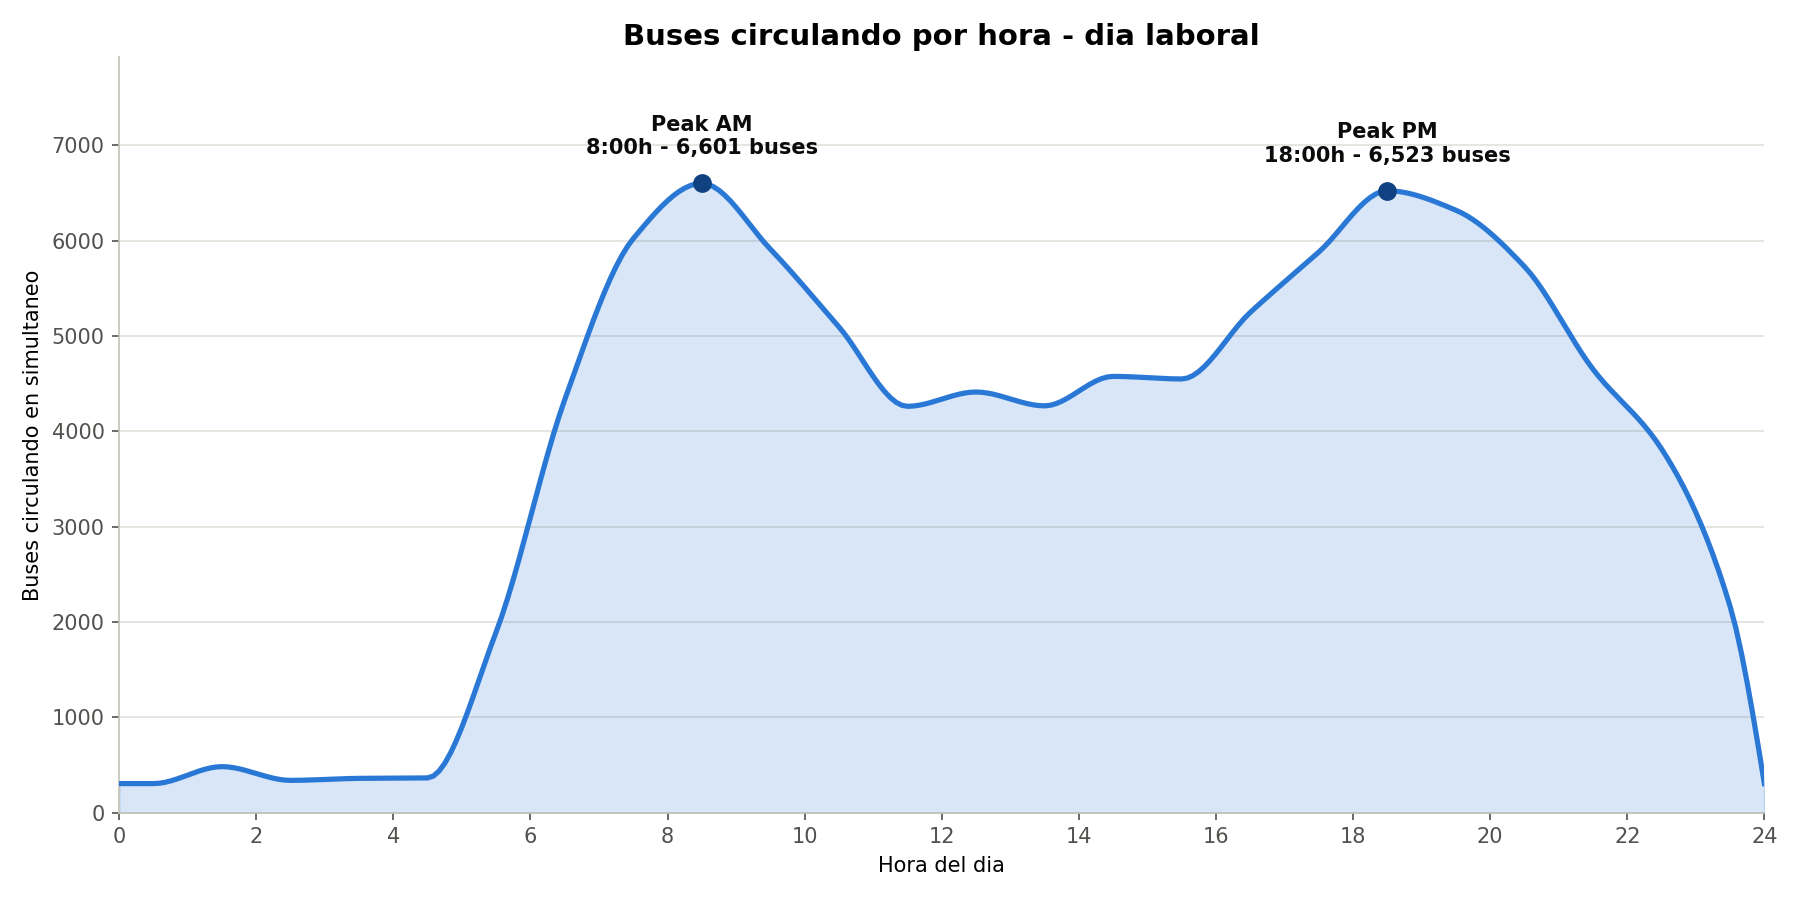
\includegraphics[width=0.65\textwidth]{./figures/buses_por_hora_curva.png}
	\caption[Buses circulando por hora]{Buses circulando por hora (d\'ia laboral)}
	\label{fig:busesporhora}
	\end{center}
\end{figure}

Esto afecta directamente a la planificaci\'on. Por una parte, la cantidad de buses necesarios para cubrir la demanda supera ampliamente la capacidad de carga simult\'anea de los electroterminales (700 espacios), por lo que las recargas deben distribuirse a lo largo del d\'ia. Por otra parte, los bloques tarifarios (Figura \ref{fig:tarifas}) tienen precios m\'as elevados justamente en las horas de mayor demanda, por lo tanto se genera una complejidad entre cubrir la demanda y minimizar el costo energ\'etico de las recargas.

\subsection{Flota e Infraestructura de Carga \label{sec:flotainfraestructura}}

La flota considerada en este proyecto es de tama\~no irrestricto y est\'a compuesta por un \'unico modelo de bus el\'ectrico, el BYD K9. La Tabla \ref{tab:especificaciones} presenta las caracter\'isticas t\'ecnicas de este veh\'iculo, las cuales definen las restricciones de autonom\'ia y recarga que deben considerarse en la planificaci\'on.

\begin{table}[htb]
\begin{center}
\small
\caption[Especificaciones t\'ecnicas bus el\'ectrico BYD K9]{Especificaciones t\'ecnicas bus el\'ectrico BYD K9}
\label{tab:especificaciones}
\begin{tabular}{@{}l r@{}}\toprule
\textbf{Par\'ametro} & \textbf{Valor} \\ \midrule
Capacidad de la bater\'ia & 350 kWh \\
Autonom\'ia m\'axima & 250 km \\
Potencia de carga & 180 kW \\
Estado de carga m\'inimo & 10\% \\
Estado de carga m\'aximo & 100\% \\
Tiempo de carga completa & 105 min \\
\bottomrule
\end{tabular}
\end{center}
\end{table}

Con una bater\'ia utilizable de 315 kWh (90\%) y un consumo de 1,4 kWh/km, la autonom\'ia real del bus es de 225 km, por lo que en jornadas extensas los buses deber\'an recargarse en electroterminales para continuar operando. La infraestructura de carga la componen 5 electroterminales distribuidos por Santiago, con una capacidad total de 700 espacios simult\'aneos.

\begin{table}[htb]
\begin{center}
\small
\caption[Capacidad de buses por electroterminal]{Capacidad de buses por electroterminal}
\label{tab:capacidadterminal}
\begin{tabular}{@{}l r@{}}\toprule
\textbf{Electroterminal} & \textbf{Capacidad} \\ \midrule
Vespucio Norte & 150 \\
El Conquistador & 180 \\
Los Espinos & 120 \\
La Reina & 100 \\
Santa Rosa & 150 \\
\midrule
Total & 700 \\
\bottomrule
\end{tabular}
\end{center}
\end{table}

Los Espinos y Santa Rosa est\'an muy cerca entre s\'i (Figura \ref{fig:mapared}), por lo que podr\'ia ser beneficioso considerarlos como un solo terminal con capacidad de 270; esta alternativa se evaluar\'a durante la ejecuci\'on del modelo.

\subsection{Costos y Tarifas \label{sec:costostarifas}}

Como vimos anteriormente, la funci\'on objetivo del problema busca minimizar el costo total de operaci\'on, el cual se compone de cuatro componentes principales. La Tabla \ref{tab:costos} resume los valores de cada costo.

\begin{table}[htb]
\begin{center}
\small
\caption[Costos operacionales del sistema]{Costos operacionales del sistema}
\label{tab:costos}
\begin{tabular}{@{}l r@{}}\toprule
\textbf{Tipo de costo} & \textbf{Precio} \\ \midrule
Costo fijo por uso de bus & 250 USD \\
Costo por minuto de espera & 0,03 USD/min \\
Costo por km recorrido & 0,5 USD/km \\
Costo fijo por recarga & 5 USD \\
\bottomrule
\end{tabular}
\end{center}
\end{table}

El costo fijo por bus incentiva a usar la menor cantidad de buses posible, dado que la flota es irrestricta. El costo por km recorrido incluye tanto los desplazamientos con pasajeros como \emph{deadheading}, \emph{pullin} y \emph{pullout}. El costo de espera penaliza los tiempos muertos entre viajes de un mismo bus, y el costo fijo por recarga se aplica cada vez que un bus entra a un electroterminal.

Adem\'as, el costo de la energ\'ia depende del periodo horario de consumo, y va desde 0,10 USD/kWh en el bloque valle (0-8h) hasta 0,22 USD/kWh en los bloques peak (14-17h y 19-22h), como muestra la Figura \ref{fig:tarifas}. El modelo debe encontrar un equilibrio entre cargar en bloques de menor costo y garantizar que todos los buses tengan energ\'ia suficiente para sus viajes asignados.

\begin{figure}[htb]
	\begin{center}
	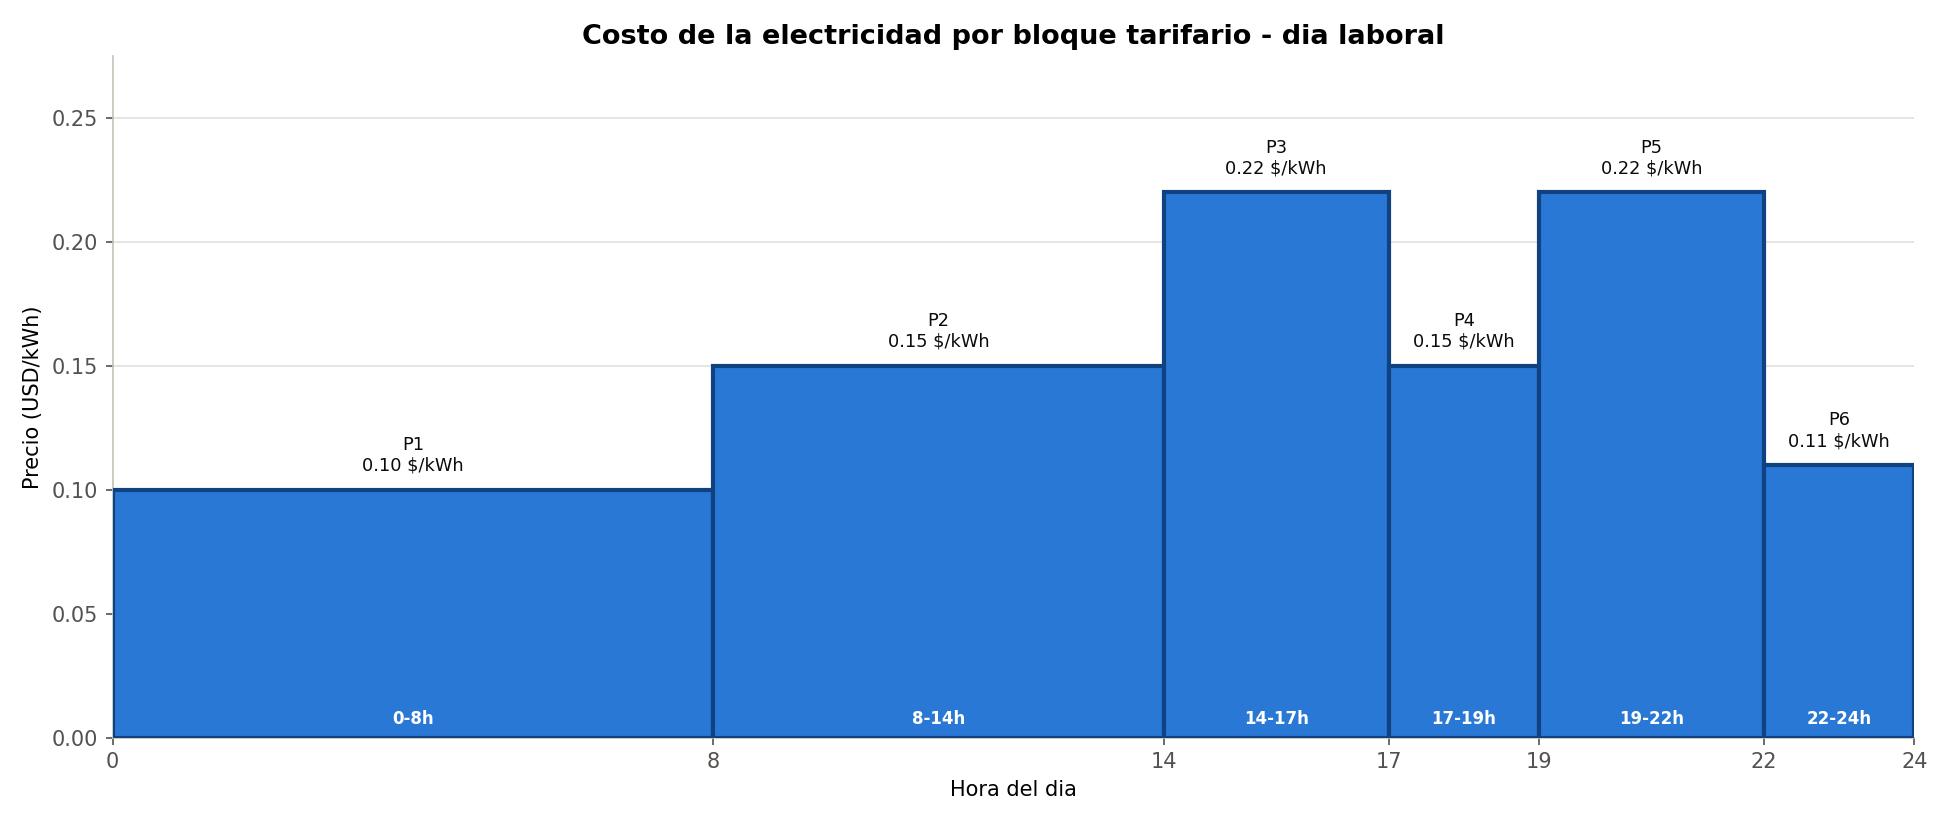
\includegraphics[width=0.6\textwidth]{./figures/costo_energia_por_periodo.png}
	\caption[Costo de la electricidad por bloque tarifario]{Costo de la electricidad por bloque tarifario (d\'ia laboral)}
	\label{fig:tarifas}
	\end{center}
\end{figure}

\subsection{Datos No Disponibles \label{sec:datosnodisponibles}}

Si bien los datos cubren la mayor parte de la informaci\'on necesaria para modelar el problema, algunos elementos no est\'an disponibles y deben aproximarse o calcularse. La duraci\'on de los viajes y las distancias de \emph{deadheading} se calculan con una velocidad promedio constante, sin considerar congesti\'on horaria ni topograf\'ia (por ejemplo, mayor pendiente en comunas precordilleranas). No se cuenta con informaci\'on de turnos de conductores, ya que el modelo planifica solo la operaci\'on del veh\'iculo, suponiendo siempre un conductor disponible. Tampoco se dispone de la demanda real de pasajeros, por lo que se usa la oferta programada (expediciones) como demanda a cumplir. Adem\'as, no existe un identificador de bloque de veh\'iculo (\texttt{block\_id}) t\'ipico de GTFS, por lo que la asignaci\'on de viajes debe construirse desde cero; tampoco hay distancias y tiempos de \emph{deadheading}, \emph{pullin} y \emph{pullout} (se calcular\'an desde la red vial de OpenStreetMap), ni energ\'ia consumida por viaje (se deriva multiplicando la distancia del trazado por el consumo de 1,4 kWh/km).

\section{KPIs \label{sec:kpis}}

Para evaluar la calidad de las soluciones generadas por el modelo, se definen cuatro indicadores de desempe\~no relevantes, alineados con el objetivo del problema.

\begin{itemize}
\item \textbf{N\'umero total de buses usados}: Indica la cantidad de buses despachados durante la jornada. Es un indicador importante para el objetivo del problema, porque la flota es de tama\~no irrestricto y cada bus utilizado incurre en un costo fijo de 250 USD.
\item \textbf{Costo energ\'etico promedio}: Se calcula como el costo total de energ\'ia dividido por los kWh totales cargados durante la jornada. Con este indicador se puede evaluar si las recargas se est\'an realizando en bloques tarifarios m\'as econ\'omicos o m\'as caros.
\item \textbf{Proporci\'on de deadheading/pullin/pullout}: Se calcula como la suma de kil\'ometros recorridos sin pasajeros (\emph{deadheading} entre viajes, \emph{pullout} desde electroterminal y \emph{pullin} de regreso) dividida por los kil\'ometros totales recorridos por la flota. Este indicador mide la eficiencia geogr\'afica de la asignaci\'on de viajes. El modelo debe buscar encadenar viajes geogr\'aficamente cercanos para minimizar este indicador.
\item \textbf{Utilizaci\'on por bus}: Se define como la raz\'on entre las horas con pasajeros y las horas totales del turno de cada bus. Con esto se eval\'ua cu\'anto del tiempo productivo de cada bus efectivamente se destina a servicio. Una utilizaci\'on alta indica que los buses pasan la mayor parte de su jornada transportando pasajeros, con tiempos de espera y recarga bien coordinados. Por el contrario, una utilizaci\'on muy baja indica problemas con la secuencia de viajes asignados.
\end{itemize}


\chapter[DISCUSI\'ON METODOL\'OGICA]{Discusi\'on Metodol\'ogica} \label{ch:metodologia}
A partir de la revisi\'on bibliogr\'afica \cite{alvo2021,perumal2022,picarelli2020,vankootenniekerk2017,zhang2024} y de las caracter\'isticas del problema, se identificaron tres alternativas metodol\'ogicas. La primera es una metaheur\'istica Adaptive Large Neighborhood Search (ALNS) que construye y mejora iterativamente una soluci\'on factible mediante operadores de destrucci\'on y reparaci\'on, con buena escalabilidad a costa de no garantizar optimalidad. La segunda combina Set Partitioning, Generaci\'on de Columnas y cortes de Benders, representando cada jornada factible como una columna y verificando que las recargas sean compatibles con la infraestructura; evita un MILP monol\'itico de gran tama\~no, aunque su implementaci\'on es m\'as compleja.

La tercera, y la seleccionada por el grupo, es una descomposici\'on espaciotemporal, que agrupa los viajes por cercan\'ia a cada electroterminal y luego los divide en ventanas horarias superpuestas resueltas por horizonte rodante, transformando el problema en subproblemas E-VSP m\'as peque\~nos resolubles con MILP directo o, en ventanas complejas, con Set Partitioning y Benders. Su beneficio es hacer tratable la escala real de RED, a costa de la optimalidad global.

\section{Metodolog\'ia 1: Adaptive Large Neighborhood Search \label{sec:metodologia1}}

Una primera alternativa ser\'ia abordar el problema mediante una metaheur\'istica de tipo Adaptive Large Neighborhood Search (ALNS). Este enfoque no garantiza la soluci\'on \'optima, sino que construye una soluci\'on inicial factible y la mejora iterativamente mediante operadores de modificaci\'on, buscando minimizar buses utilizados, costos operacionales y desplazamientos sin pasajeros, explorando el espacio de soluciones de forma heur\'istica en lugar de con una formulaci\'on matem\'atica exacta. As\'i, sacrifica algo de optimalidad a cambio de eficiencia computacional.

Una soluci\'on corresponde a la asignaci\'on completa de viajes y decisiones de carga a cada bus (el conjunto de jornadas vigentes en un momento del algoritmo). El proceso parte de una regla simple (asignar los viajes en orden de horario al primer bus disponible que pueda ejecutarlos sin quedar sin bater\'ia, despachando uno nuevo si ninguno puede hacerlo). Sobre esta soluci\'on se aplican iterativamente un operador de destrucci\'on, que remueve viajes con mayor desplazamiento sin pasajeros o conflicto de carga, y uno de reparaci\'on, que reinserta esos viajes en la posici\'on de menor costo que preserve horarios, bater\'ia y capacidad de carga (agregando un bus nuevo solo si es necesario). La nueva soluci\'on se acepta si mejora la actual, y ocasionalmente aunque empeore, con probabilidad decreciente, para evitar quedar atrapado en una soluci\'on de baja calidad. El ciclo se repite hasta un criterio de t\'ermino, priorizando los operadores con mejores resultados recientes.

Esta metodolog\'ia ha sido aplicada con \'exito a problemas de estructura similar al nuestro: \citeA{wang2024} dise\~nan un ALNS para un problema con m\'ultiples electroterminales y restricciones de infraestructura de carga, con operadores de destrucci\'on y reparaci\'on adaptados al problema (por ejemplo, priorizar la remoci\'on de viajes con mayor holgura horaria, o reconstruir las jornadas de mayor costo promedio) y un mecanismo de aceptaci\'on tipo recocido simulado. En su experimento, el algoritmo alcanza una primera soluci\'on factible en 13,6 minutos y sigue mejor\'andola de forma consistente, demostrando que el enfoque genera soluciones de buena calidad en tiempos razonables pese a la alta complejidad combinatoria del problema conjunto de asignaci\'on y carga.

Los datos disponibles son consistentes con los supuestos de esta metodolog\'ia, ya que se tienen cinco electroterminales, validando el car\'acter multi-electroterminal del problema, y se dispone de la informaci\'on de capacidad de cargadores, par\'ametros de bater\'ia y tarifas necesaria para modelar las restricciones de carga. Dada la escala real del problema (417 rutas y 64.502 expediciones), una implementaci\'on completa probablemente se beneficiar\'ia de una descomposici\'on previa por zona o ventana horaria, siguiendo a \citeA{zhou2024}, quienes combinan un m\'etodo exacto para subproblemas peque\~nos con ALNS para la escala completa en la red de Singapur (m\'ultiples electroterminales y flota heterog\'enea).

\section{Metodolog\'ia 2: Set Partitioning con Generaci\'on de Columnas y Cortes de Benders \label{sec:metodologia2}}

Otra alternativa consiste en formular el problema mediante Set Partitioning y resolverlo utilizando Generaci\'on de Columnas, complementada con una verificaci\'on de los itinerarios de carga mediante cortes de Benders. Esta metodolog\'ia busca determinar la cantidad de buses el\'ectricos requerida y seleccionar un conjunto de jornadas que permita cubrir exactamente una vez todos los viajes entregados por la planificaci\'on, minimizando la cantidad de buses utilizados, los costos operacionales asociados y los desplazamientos sin pasajeros.

La metodolog\'ia se entiende como una con dos niveles de decisi\'on. En el primero se seleccionan las jornadas de buses mediante Set Partitioning y Generaci\'on de Columnas. En el segundo se verifica y programa el itinerario conjunto de carga.

Cada columna generada corresponde a una jornada completa propuesta para un bus, con sus secuencias de viajes, desplazamientos en vac\'io y periodos de espera, junto con la evoluci\'on de bater\'ia durante todo el recorrido (por ejemplo, salida del electroterminal, varios viajes consecutivos, una recarga y el retorno). Estas columnas deben ser individualmente factibles en horarios, energ\'ia y ubicaciones, pero no determinan la hora exacta ni el cargador a utilizar, ya que eso depende de la necesidad de carga conjunta de todos los buses.

Como visi\'on preliminar de la formulaci\'on, la principal variable de decisi\'on del problema maestro ser\'a binaria e indicar\'a si una determinada jornada factible es seleccionada o no:
\begin{equation}
Y_j = \begin{cases} 1 & \text{si se selecciona la jornada } j \\ 0 & \text{en caso contrario} \end{cases}
\label{eq:variabley}
\end{equation}

La restricci\'on fundamental de Set Partitioning exigir\'a que cada viaje programado pertenezca exactamente a una de las jornadas seleccionadas:
\begin{equation}
\sum_{j} a_{ij}\, Y_j = 1 \qquad \forall i
\label{eq:setpartitioning}
\end{equation}

Adicionalmente, el subproblema de carga deber\'a asegurar que las recargas programadas no superen simult\'aneamente la capacidad disponible de cada electroterminal, y por ende que las necesidades de carga e itinerarios creados sean posibles de cumplir con la capacidad conjunta de los cinco electroterminales.

El problema maestro selecciona la combinaci\'on de columnas de menor costo que cubre todos los viajes una vez. Dada la gran cantidad de jornadas posibles, la Generaci\'on de Columnas parte de un conjunto reducido y resuelve una versi\'on restringida del problema maestro; un subproblema busca nuevas columnas que mejoren la soluci\'on actual y las agrega solo si lo logran, repitiendo el procedimiento.

Una vez obtenida una soluci\'on candidata, un subproblema tipo Benders verifica si sus requerimientos de carga pueden satisfacerse con la infraestructura disponible en cada momento, determinando horarios, ubicaci\'on y duraci\'on de carga de cada bus. Aunque cada jornada sea factible individualmente, su combinaci\'on puede no serlo si excede la carga disponible en algún terminal; de detectarse esa infactibilidad, se genera un corte que se incorpora al problema maestro para evitar volver a seleccionar ese conjunto de columnas.

\textbf{Aspectos positivos:}
\begin{itemize}
\setlength{\itemsep}{1pt}
\item Descompone un problema de gran escala en componentes manejables, evitando resolver simult\'aneamente todas las decisiones de viajes y carga.
\item Set Partitioning representa de forma natural la operaci\'on de cada bus mediante jornadas completas (viajes, desplazamientos sin pasajeros, espera y evoluci\'on de bater\'ia).
\item La Generaci\'on de Columnas evita enumerar todas las jornadas factibles, generando solo las que contribuyen a mejorar la soluci\'on.
\item El subproblema tipo Benders separa las restricciones compartidas de carga, verificando compatibilidad con la infraestructura disponible.
\end{itemize}

\textbf{Aspectos negativos:}
\begin{itemize}
\setlength{\itemsep}{1pt}
\item Alta complejidad de implementaci\'on, pues exige coordinar iterativamente un problema maestro, un subproblema de columnas y un subproblema de factibilidad de carga.
\item Las restricciones compartidas entre buses (capacidad simult\'anea de cargadores) pueden provocar m\'ultiples iteraciones antes de una planificaci\'on globalmente factible.
\item Al trabajar inicialmente sobre la relajaci\'on lineal, obtener una soluci\'on entera puede requerir etapas adicionales, haciendo su desarrollo computacional m\'as exigente que un MILP directo.
\end{itemize}

\section{Metodolog\'ia Propuesta: Descomposici\'on Espaciotemporal \label{sec:metodologiapropuesta}}

La metodolog\'ia que proponemos consiste en descomponer el problema espacial y temporalmente. En lugar de optimizar simult\'aneamente todos los viajes de la red, se segmentan y agrupan en torno a los cinco electroterminales, considerando el lugar de inicio y t\'ermino de cada viaje, su distancia al electroterminal, los desplazamientos sin pasajeros (\emph{deadheads}) y su compatibilidad con otros viajes. Luego, cada bloque de recorridos por electroterminal se descompone en subproblemas por horas, cada uno resolviendo la asignaci\'on de viajes y el programa de carga para las paradas dentro de esa ventana.

Existe evidencia que respalda ambas descomposiciones; el desaf\'io est\'a en combinarlas. La descomposici\'on espacial es un principio cl\'asico en problemas VSP/VRP de gran escala, y consiste en agrupar primero los viajes por ubicaci\'on/terminal y luego resolver el ruteo de cada grupo por separado. \citeA{gao2024} utilizan esta idea en un MDVSP (multidep\'osito) similar al nuestro, asignando inicialmente los viajes a un dep\'osito, resolviendo el problema por dep\'osito y repitiendo el procedimiento tras ajustar el agrupamiento hasta obtener una soluci\'on satisfactoria; este enfoque es replicable a las electroterminales de nuestro problema.

La descomposici\'on temporal es m\'as dif\'icil, por lo complicado de unir soluciones que quedan atravesadas entre los l\'imites de los intervalos. \citeA{kim2023} muestran por qu\'e cortar el tiempo en bloques fijos es riesgoso, y proponen en cambio crear intervalos de tiempo superpuestos y resolver mediante un enfoque de horizonte rodante, iterando sobre una secuencia de intervalos superpuestos en vez de bloques disjuntos.

Para el desarrollo del m\'etodo proponemos estructurarlo en dos fases, cada una con su propio problema de optimizaci\'on.

\subsection{Fase 1: Asignaci\'on Espacial \label{sec:fase1}}

Se formula un problema de asignaci\'on de transporte con una variable binaria que indica si un viaje se asigna a un electroterminal (uno y solo uno por viaje). El costo se define por el \emph{deadhead} de ida m\'as el de vuelta al terminal, asignando el de menor costo (aproximado, pues el viaje podr\'ia encadenarse con otro antes de volver); la capacidad de cada terminal viene de \texttt{charging\_activities.csv}. El objetivo es minimizar el \emph{deadhead} total, balanceando la carga entre los cinco electroterminales. Este problema es resoluble como una LP de transporte relajada, muy r\'apida; como una asignaci\'on de una sola pasada puede alejarse del \'optimo, se busca modificar el agrupamiento, de ser necesario, y repetir el proceso hasta lograr una distribuci\'on m\'as equitativa.

\subsection{Fase 2: Descomposici\'on Temporal \label{sec:fase2}}

Dada una asignaci\'on por bloques de viajes para cada electroterminal, se corta el d\'ia en ventanas de tiempo superpuestas de 3 horas que avanzan de a 1 hora (0:00--3:00, 1:00--4:00, 2:00--5:00, \ldots). El avance de 1 hora asegura que el l\'imite izquierdo de cada ventana caiga en una hora exacta, coherente con la granularidad de los bloques tarifarios de \texttt{charging\_activities.csv}, y que la primera hora de cada ventana, cuya soluci\'on se fija definitivamente, coincida con el inicio de un bloque tarifario, mientras las dos horas restantes quedan como horizonte flexible que se reoptimiza en la siguiente iteraci\'on. El largo de 3 horas responde a que los buses demoran 105 minutos (1:45 hrs) en cargar, por lo que para fijar la primera hora el modelo debe poder ``ver hacia el futuro'' hasta que los buses terminen de cargar. Al resolver cada ventana, solo se fija la primera hora; las dos horas siguientes act\'uan como borrador que se reoptimiza en la iteraci\'on siguiente, con m\'as informaci\'on de los pr\'oximos viajes. El estado de cada bus (ubicaci\'on, nivel de bater\'ia) se transmite como condici\'on inicial a la siguiente ventana.

Cada subproblema de la Fase 2 es una instancia peque\~na de E-VSP, correspondiente a un electroterminal por una ventana horaria, la cual puede ser resuelta con MILP directo o mezclarse con la Metodolog\'ia 1 y resolverse mediante Set Partitioning + Generaci\'on de Columnas, dado que est\'a a una escala reducida y las columnas son manejables.

Como apoyo a la propuesta, se realiz\'o una prueba de la asignaci\'on espacial de las 64.502 expediciones de los d\'ias laborales.

\begin{figure}[htb]
	\begin{center}
	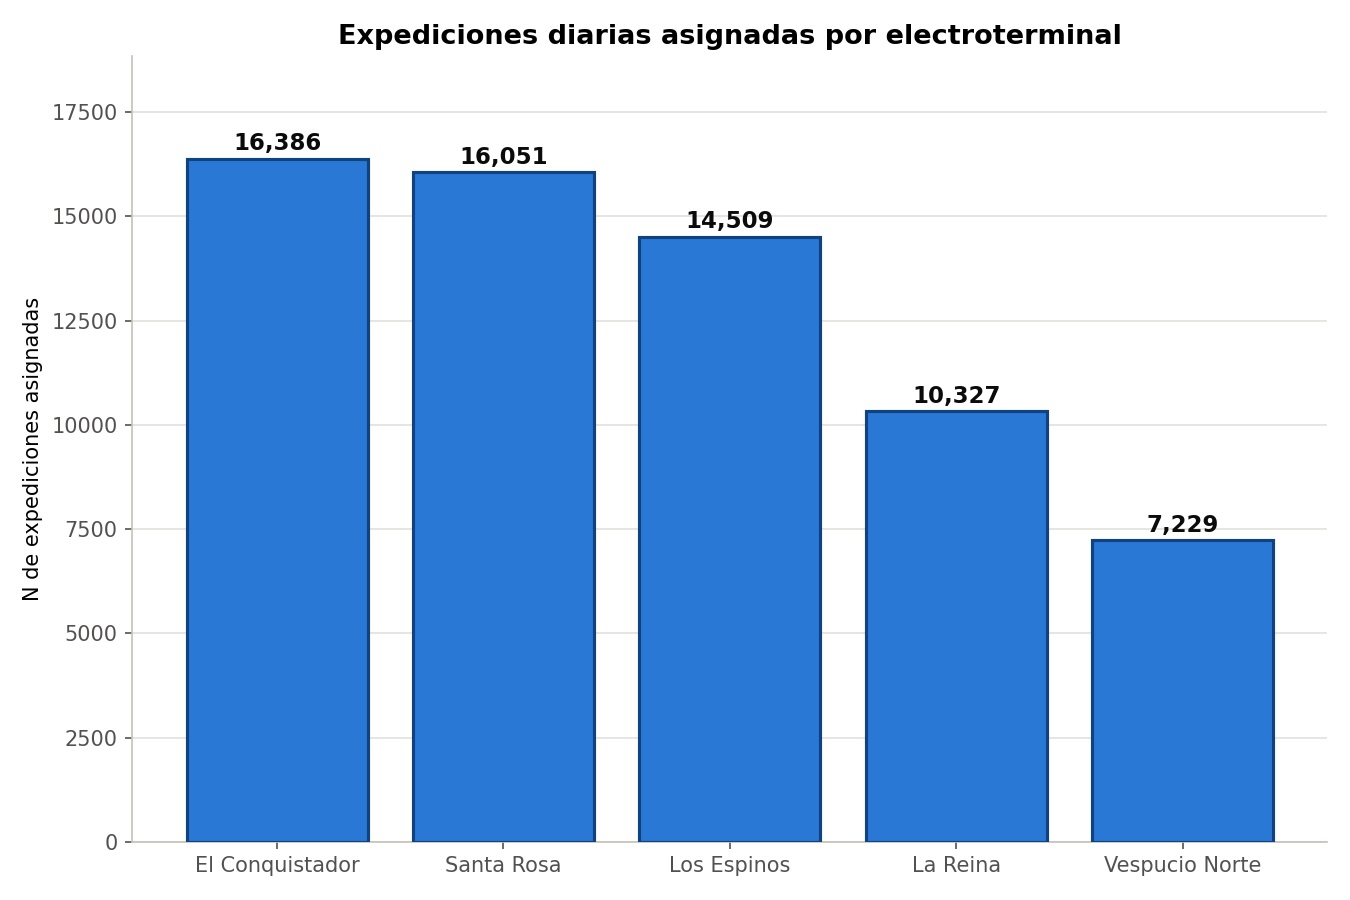
\includegraphics[width=0.55\textwidth]{./figures/expediciones_por_electroterminal.jpg}
	\caption[Expediciones diarias asignadas por electroterminal]{Expediciones diarias asignadas por electroterminal}
	\label{fig:expedicionesterminal}
	\end{center}
\end{figure}

Como se observa en la Figura \ref{fig:expedicionesterminal}, esta asignaci\'on distribuye las expediciones en cinco conjuntos de tama\~no reducido, transformando el problema completo en cinco problemas menores. Sin embargo, no asegura una asignaci\'on \'optima y puede restringir la concatenaci\'on de expediciones \'optimas, por lo que debe validarse y, de ser necesario, ajustar el criterio de asignaci\'on.

\textbf{Aspectos positivos:}
\begin{itemize}
\setlength{\itemsep}{1pt}
\item Reduce el problema de 64.502 expediciones / 5 electroterminales / 1 d\'ia a m\'ultiples subproblemas manejables, cada uno resoluble de forma exacta.
\item El uso de tarifas horarias encaja bien con la descomposici\'on temporal, ya que cada ventana sabe en qu\'e bloque de tarifas est\'a.
\item Puede integrarse con la Metodolog\'ia 2, ya que las ventanas de mayor complejidad (por ejemplo, las que calcen con horarios peak) pueden resolverse con Generaci\'on de Columnas y cortes de Benders.
\end{itemize}

\textbf{Aspectos negativos:}
\begin{itemize}
\setlength{\itemsep}{1pt}
\item Se pierde la garant\'ia de optimalidad global, ya que una mala asignaci\'on en la Fase 1 o una decisi\'on sub\'optima en la Fase 2 no se corrige salvo que se agregue un paso de reparaci\'on.
\item La calidad depende fuertemente del tama\~no de ventana, pues ventanas muy cortas empeoran la calidad, y muy largas devuelven el problema a lo original.
\item Alta complejidad de dise\~no, especialmente al decidir qu\'e informaci\'on del futuro pasar a cada subproblema para evitar decisiones que resulten infactibles m\'as adelante.
\end{itemize}

Dada esta complejidad, se planea una implementaci\'on progresiva, comenzando con versiones simplificadas del problema e incorporando gradualmente las restricciones hasta la formulaci\'on completa. Como estrategia alternativa, si la metodolog\'ia resulta demasiado exigente computacionalmente, se propone sacrificar la descomposici\'on temporal y centrarse principalmente en la asignaci\'on espacial de los viajes.


\chapter[CONCLUSIONES]{Conclusiones}
\section{Conclusiones Relevantes \label{sec:conclusionesrelevantes}}

Este informe presenta una primera aproximaci\'on al problema de planificaci\'on operacional de la flota de buses el\'ectricos de RED, formulado como un Electric Vehicle Scheduling Problem (E-VSP). Se caracteriz\'o el problema en sus tres decisiones centrales, asignaci\'on de viajes a buses, desplazamientos sin pasajeros y programaci\'on de recargas, y se estableci\'o como objetivo minimizar el costo total de operaci\'on sujeto a la cobertura completa de los viajes y a las restricciones de autonom\'ia, horario y capacidad de carga.

El an\'alisis de datos confirm\'o la magnitud del desaf\'io: un d\'ia laboral concentra 417 rutas y 64.502 expediciones, con dos peaks de demanda (8:00 y 18:00) que superan ampliamente la capacidad de carga simult\'anea de los cinco electroterminales (700 espacios) y que coinciden parcialmente con los bloques tarifarios m\'as caros. Esto valida que el problema exige coordinar conjuntamente las decisiones de transporte y de energ\'ia, y no puede resolverse como una simple asignaci\'on de viajes.

La revisi\'on bibliogr\'afica permiti\'o identificar tres enfoques metodol\'ogicos viables (ALNS, Set Partitioning con Generaci\'on de Columnas y Benders, y descomposici\'on espaciotemporal), cada uno con ventajas y limitaciones distintas en escalabilidad, calidad de soluci\'on y complejidad de implementaci\'on. Se seleccion\'o la descomposici\'on espaciotemporal como metodolog\'ia principal por su capacidad de reducir la escala real del problema a subproblemas manejables (asignaci\'on espacial por electroterminal seguida de ventanas horarias superpuestas), manteniendo la posibilidad de integrarse con la segunda metodolog\'ia en los tramos m\'as complejos.

Esta etapa preliminar permiti\'o sentar las bases conceptuales, de datos y metodol\'ogicas del proyecto. El desaf\'io de las siguientes etapas ser\'a traducir esta propuesta en una implementaci\'on computacional concreta, validarla con los datos reales de RED y evaluar si el enfoque logra un equilibrio adecuado entre tratabilidad computacional y calidad de la soluci\'on obtenida.

\section{Pasos Futuros \label{sec:pasosfuturos}}

Habiendo descrito el problema, analizado los datos disponibles y seleccionado la metodolog\'ia de descomposici\'on espaciotemporal como enfoque principal, el trabajo futuro se estructurar\'a en cinco etapas secuenciales:

\begin{enumerate}
\item \textbf{Formular el modelo por fases.} Se desarrollar\'a la formulaci\'on matem\'atica completa de la metodolog\'ia propuesta, separando expl\'icitamente la Fase 1 (asignaci\'on espacial de viajes a electroterminales) y la Fase 2 (descomposici\'on temporal mediante ventanas superpuestas y horizonte rodante). Esto incluye definir con precisi\'on las variables de decisi\'on, la funci\'on objetivo y el conjunto completo de restricciones (cobertura de viajes, factibilidad horaria, evoluci\'on de bater\'ia, capacidad de carga simult\'anea) para cada subproblema.
\item \textbf{Implementar la modelaci\'on computacional.} Se traducir\'a la formulaci\'on a un modelo ejecutable, utilizando un solver de optimizaci\'on (MILP) para los subproblemas de la Fase 2, junto con las rutinas necesarias para la asignaci\'on espacial de la Fase 1 y la transmisi\'on del estado de cada bus (ubicaci\'on, nivel de bater\'ia) entre ventanas consecutivas.
\item \textbf{Probar con datos de RED.} El modelo se ejecutar\'a sobre el caso base ya construido (d\'ia laboral, 417 rutas, 64.502 expediciones), comenzando con instancias reducidas o electroterminales individuales para verificar el correcto funcionamiento del modelo antes de escalarlo a la red completa.
\item \textbf{Validar y ajustar par\'ametros.} Se evaluar\'a la sensibilidad de la soluci\'on al tama\~no de las ventanas temporales, al criterio de agrupamiento espacial en la Fase 1 y a los costos definidos, ajustando estos par\'ametros en caso de detectar infactibilidades recurrentes o soluciones de baja calidad. En esta etapa tambi\'en se evaluar\'a la alternativa de fusionar los electroterminales Los Espinos y Santa Rosa, y se decidir\'a si es necesario incorporar Set Partitioning con Generaci\'on de Columnas y cortes de Benders en las ventanas horarias de mayor complejidad (horas peak).
\item \textbf{Analizar resultados y presentarlos.} Finalmente, se construir\'an los entregables definidos en la Secci\'on \ref{sec:entregable} (jornadas por bus, itinerario de carga, desglose de costos), se calcular\'an los KPIs definidos en la Secci\'on \ref{sec:kpis} y se compararan los resultados obtenidos contra los del caso base, documentando las conclusiones y limitaciones del enfoque para la presentaci\'on final.
\end{enumerate}

La Tabla \ref{tab:gantt} presenta la Carta Gantt planificada para estas cinco etapas a lo largo de las diez semanas siguientes.

\begin{table}[htb]
\begin{center}
\caption[Carta Gantt de trabajo futuro]{Carta Gantt de trabajo futuro}
\label{tab:gantt}
\resizebox{\textwidth}{!}{%
\begin{tabular}{@{}l *{10}{c}@{}}\toprule
\textbf{Actividad} & \textbf{S1} & \textbf{S2} & \textbf{S3} & \textbf{S4} & \textbf{S5} & \textbf{S6} & \textbf{S7} & \textbf{S8} & \textbf{S9} & \textbf{S10} \\ \midrule
Formular el modelo de optimizaci\'on & \cellcolor{ganttgreen} & \cellcolor{ganttgreen} & & & & & & & & \\
Implementar y validar modelo simplificado & & \cellcolor{ganttgreen} & \cellcolor{ganttgreen} & & & & & & & \\
Incorporar restricciones progresivamente & & & \cellcolor{ganttgreen} & \cellcolor{ganttgreen} & \cellcolor{ganttgreen} & \cellcolor{ganttgreen} & & & & \\
Implementar descomposici\'on temporal & & & & & & \cellcolor{ganttgreen} & \cellcolor{ganttgreen} & & & \\
Integrar metodolog\'ia completa & & & & & & & \cellcolor{ganttgreen} & \cellcolor{ganttgreen} & & \\
Escalar metodolog\'ia para caso RED & & & & & & & & \cellcolor{ganttgreen} & \cellcolor{ganttgreen} & \\
Analizar resultados y ajustar par\'ametros & & & & & & & & & \cellcolor{ganttgreen} & \cellcolor{ganttgreen} \\
\bottomrule
\end{tabular}%
}
\end{center}
\end{table}


%%%%%%%%%%%%%
%       REFERENCES        %
%%%%%%%%%%%%%

\cleardoublepage
\phantomsection \label{references}
\bibliographystyle{apacite}
\renewcommand{\bibname}{BIBLIOGRAF\'IA}

%%%% ACTIVAR SIGUIENTES 3 LINEAS SI POSTGRADO RECHAZA LA BIBLIOGRAFIA
%\setlength{\bibleftmargin}{0em}
%\setlength{\bibindent}{0em}
%\setlength{\bibitemsep}{1em}

\setlength{\bibitemsep}{0.3em}
{\small\singlespacing\bibliography{Thesis}}

%%%%%%%%%%%%
%      ANEXOS      %
%%%%%%%%%%%%

\appendix % Cada anexo (A, B, C...) se declara como \section

\newpage
\section[Anexo 1: Declaraci\'on de Uso de IA]{Anexo 1: Declaraci\'on de Uso de Inteligencia Artificial en este Informe y Presentaci\'on Asociada}
% Espacio reservado para las fotos/escaneos de las firmas de cada integrante.
% Instrucciones completas en la Guia de Entrega. Para activar una firma,
% guarda la foto como PNG o JPG con el nombre exacto indicado en cada
% \firmaBox (segundo argumento) dentro de la carpeta ./firmas/.
% Mientras el archivo no exista, se mostrara un recuadro con "(firma pendiente)".
\newcommand{\firmaBox}[2]{%
  \begin{minipage}[t]{4.6cm}
    \centering
    \IfFileExists{./firmas/#2.png}%
      {\includegraphics[width=4cm,height=2.2cm,keepaspectratio]{./firmas/#2.png}}%
      {\IfFileExists{./firmas/#2.jpg}%
        {\includegraphics[width=4cm,height=2.2cm,keepaspectratio]{./firmas/#2.jpg}}%
        {\IfFileExists{./firmas/#2.jpeg}%
          {\includegraphics[width=4cm,height=2.2cm,keepaspectratio]{./firmas/#2.jpeg}}%
          {\fbox{\begin{minipage}[c][2.2cm][c]{3.9cm}\centering\footnotesize\textit{(firma pendiente)}\end{minipage}}}%
        }%
      }\\[2pt]
    \rule{4cm}{0.4pt}\\[2pt]
    \small #1
  \end{minipage}%
}

\noindent \textbf{Grupo:} 24

\vspace{0.5cm}

\noindent \textbf{\textquestiondown Hicieron uso de herramientas de IA en su trabajo para este informe y/o presentaci\'on?} \\
SI $\boxtimes$ \hspace{1.5cm} NO $\square$

\vspace{0.5cm}

\noindent \textbf{\textquestiondown Cu\'ales de las siguientes alternativas describen mejor el uso que hicieron de IA?} (puede marcarse m\'as de una)

\vspace{0.2cm}

\begin{itemize}
\setlength{\itemsep}{2pt}
\item[$\boxtimes$] Apoyo a la redacci\'on, ortograf\'ia, estructura gramatical, etc., de los documentos.
\item[$\boxtimes$] Apoyo al an\'alisis de datos e informaci\'on asociada al problema.
\item[$\boxtimes$] B\'usqueda y/o filtro de referencias, contenidos web, literatura, etc., relevante al proyecto.
\item[$\square$] Apoyo para el desarrollo de modelos asociados al proyecto.
\item[$\boxtimes$] Apoyo en el desarrollo de c\'odigo computacional necesario para el proyecto.
\item[$\square$] Apoyo en el an\'alisis de resultados (por ejemplo, de distintas corridas computacionales, tendencias de predicciones, etc.).
\item[$\square$] Apoyo para construir figuras, diagramas, etc.
\item[$\boxtimes$] Apoyo para obtener conclusiones a partir de los an\'alisis de resultados.
\item[$\square$] Otro, especificar: \rule{6cm}{0.4pt}
\end{itemize}

\vspace{0.3cm}

\noindent \textbf{Indiquen qu\'e chats de IA usaron y una breve reflexi\'on respecto al uso de IA:}

\vspace{0.2cm}

\noindent Se utiliz\'o Claude (Sonnet 4.6), ChatGPT (GPT-5.6 ``Luna'') y Qwen3.7 Plus. Fue un apoyo bastante \'util en t\'erminos de eficiencia, al trabajar con una extensa cantidad de datos. Fue importante para la creaci\'on de scripts para obtener gr\'aficos, la interpretaci\'on de resultados en el an\'alisis de datos y la redacci\'on del informe. No consideramos que haya sido indispensable su uso para la realizaci\'on de esta Entrega 1, pero s\'i definitivamente ayud\'o a acortar el tiempo que llev\'o el trabajo y a mitigar la cantidad de errores humanos, como inconsistencias o faltas de ortograf\'ia. Tambi\'en se utiliz\'o Claude (Sonnet 5) para traspasar el contenido ya redactado por el grupo al formato LaTeX de la plantilla del curso, generando los archivos .tex del informe. Adicionalmente, Claude (Sonnet 5) fue clave para ajustar el informe al l\'imite de p\'aginas de la entrega, ya que ayud\'o a reducirlo de 28 a 20 p\'aginas, lo que implic\'o reescribir buena parte de la redacci\'on original del grupo con redacci\'on generada por esta IA.

\vspace{1cm}

\noindent \textbf{Esta declaraci\'on debe ser firmada por todos los integrantes del grupo:}

\vspace{0.8cm}

\begin{center}
\begin{tabular}{ccc}
\firmaBox{Nicol\'as Bennett}{nicolas_bennett} & \firmaBox{Antonio De Frutos}{antonio_defrutos} & \firmaBox{Claudio Hasb\'un}{claudio_hasbun} \\[1.1cm]
\firmaBox{Agust\'in Irarr\'azaval}{agustin_irarrazaval} & \firmaBox{Joaqu\'in Jim\'enez}{joaquin_jimenez} & \firmaBox{Alonso Muelas}{alonso_muelas} \\
\end{tabular}
\end{center}


\newpage
\section[Anexo 2: Datos Disponibles]{Anexo 2: Detalle de los Datos Disponibles}
Como material complementario a la Secci\'on \ref{sec:datosdisponibles} (Datos Disponibles), la Tabla \ref{tab:datosdisponibles} detalla cada archivo de datos utilizado en el proyecto, su contenido y el uso espec\'ifico que se le dar\'a durante la modelaci\'on.

\begin{table}[H]
\begin{center}
\small
\caption[Datos disponibles]{Datos disponibles}
\label{tab:datosdisponibles}
\begin{tabular}{@{}p{0.30\textwidth} p{0.35\textwidth} p{0.25\textwidth}@{}}\toprule
\textbf{Archivo} & \textbf{Contenido} & \textbf{Uso en el proyecto} \\ \midrule
GTFS (routes, trips, stop\_times, frequencies, stops, shapes) & Rutas, viajes, horarios, paraderos y trazados & Demanda programada \\
shape\_distances.csv & Distancia por trazado & C\'alculo de energ\'ia \\
chile.gpkg & Red vial de Chile & C\'alculo de distancias sin pasajeros \\
depots.csv & Ubicaci\'on y capacidad de electroterminales & Infraestructura de carga \\
charger\_capacity.csv & Capacidad de carga simult\'anea & Restricci\'on de carga \\
electricity\_prices.csv & Tarifas por bloque horario & Costo energ\'etico \\
vehicles.csv & Par\'ametros de bus BYD K9 & Informaci\'on flota \\
parameters.csv & Costos y par\'ametros globales & Funci\'on objetivo \\
\bottomrule
\end{tabular}
\end{center}
\end{table}


\end{document}
